% ---
% tags: [注意力, 稀疏注意力, 线形注意力]
% author: marshall
% excerpt:
% ---
\documentclass[11pt]{article}

\usepackage{fontspec}
\usepackage{xeCJK}
% macOS 上 SimSun 位于 Microsoft Word 内部；如需其它字体请修改下面路径
\setCJKmainfont[Path=/Applications/Microsoft Word.app/Contents/Resources/DFonts/, Extension=.ttc]{Simsun}

\usepackage[a4paper, margin=2.2cm]{geometry}
\linespread{1.3}
\setlength{\parskip}{0.3em}
\usepackage{amsmath, amssymb, amsthm}
\usepackage{graphicx}
% 本文图片统一放在与 .tex 同名的文件夹 latex/<slug>/ 中，直接用文件名引用即可
\graphicspath{{./}{2026-11-23-sparse-linear-attention/}}
\usepackage{hyperref}
\hypersetup{colorlinks=true, linkcolor=blue, urlcolor=blue}

\title{浅析稀疏/线形注意力路线之争}
\author{Marshall}

\begin{document}
\maketitle

当现代 LLM 的上下文窗口向着 1M 扩展的时候，标准 Softmax Attention 的 $O(N^2)$ 算力成本和线形的 KV Cache 显存开销逐渐变得难以让人接受，目前逐渐收敛到了两条技术路线：

\begin{itemize}
  \item 稀疏注意力（Sparse）：选择部分位置的 KV Cache 进行计算。
  \item 线形注意力（Linear）：通过状态压缩，将历史信息压缩进一个固定大小的状态矩阵。
\end{itemize}

\section{评析视角与方法论}

本文主要从以下角度来分析不同技术路线的优劣势：

\begin{enumerate}
  \item \textbf{计算开销}：这里主要的口径是单位 Query 与单位 History 之间的计算成本，即处理一个 Query 需要与多少历史信息进行交互，以及每次交互所需的计算量。
  \item \textbf{显存开销}：主要关注 KV Cache 或状态矩阵的存储规模，以及其随上下文长度增长的变化趋势。对于长上下文场景，除了静态显存占用，还需要考虑 KV Cache 的读写带宽和显存访问效率。
  \item \textbf{精度损失}：显而易见的是，无论是稀疏注意力还是线形注意力，其相比于全注意力肯定是有一些精度损失的，只是损失来源不同：
    \begin{itemize}
      \item Sparse Attention 主要面临信息筛选与访问受限带来的问题，如窗口边界效应（Window Boundary Effect）、长距离依赖丢失和注意力分布偏移（Attention Distribution Shift）；
      \item Linear Attention 则主要面临有限状态容量带来的信息压缩与记忆问题，如记忆干扰（Memory Interference）、历史信息遗忘（Memory Forgetting）和精确信息检索能力下降。
    \end{itemize}
  \item \textbf{硬件友好程度}：主要考虑是否能够充分利用 GPU 等现代加速器的计算能力，包括矩阵乘法的规整程度、访存连续性、计算并行度，以及对 Tensor Core 等专用计算单元的利用情况。
  \item \textbf{通用 feature 支持度}：现代 LLM 技术已经形成了一套庞杂的系统，除了 Attention 骨架本身，我们更多也要考虑其与其他技术架构的结合友好程度，包括 Prefix Cache、KV Cache 量化与 Offload、Paged KV Cache、变长序列、分布式推理等工程特性的支持情况。
\end{enumerate}

\section{稀疏注意力}

值得注意的是，稀疏注意力有非常多的形式变体，笼统地来讲，只要涉及到“选择一部分”来进行计算，就符合“稀疏”的字面定义，以下挑一些经典的架构来分析，但不代表稀疏注意力就只有这么几个范式，其实各种排列组合和稀疏方式是非常多样化的。

\subsection{NSA}

NSA（Native Sparse Attention）希望让模型根据当前 Query 的需求，自适应地选择值得访问的历史信息。它的一个重要设计思路是：\textbf{不同粒度的历史信息应该采用不同的访问方式。}

例如，对于距离当前 Query 较近的 Token，通常需要保留细粒度的信息；对于距离较远的历史上下文，则可以通过压缩或聚合的方式降低访问成本。核心设计分为以下三个组件，同一个 Query 构建三条并行的 Attention 分支：

\begin{enumerate}
  \item \textbf{Compression（压缩注意力）}

  将连续的多个 Token 压缩成一个代表性的 KV 表示，通过可学习的 MLP 完成块级信息聚合。这样，Query 不需要逐个访问历史 Token，就能获得整个上下文的粗粒度信息。

  \begin{figure}[htbp]
    \centering
    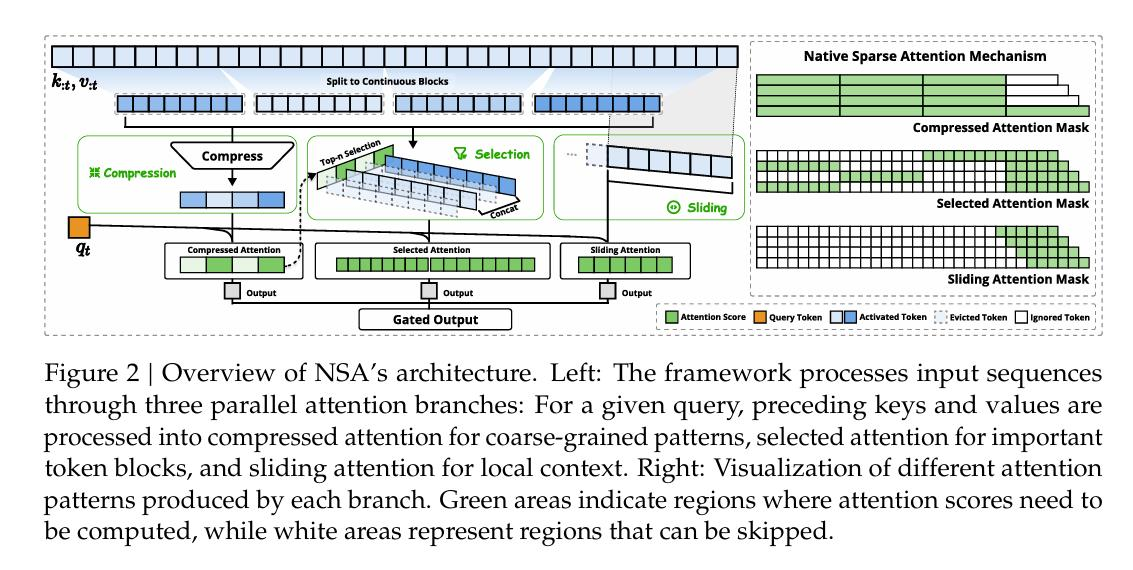
\includegraphics[width=0.8\textwidth]{nsa-compression.png}
    \caption{NSA 的压缩注意力分支}
    \label{fig:nsa-compression}
  \end{figure}

  \item \textbf{Selection（选择注意力）}

  利用 Compression 分支计算得到的注意力分数，对历史 Block 进行重要性排序，选择 Top-$n$ 个 Block，再从原始 KV Cache 中取出这些 Block 的完整 KV，进行精确 Attention 计算。

  \item \textbf{Sliding（滑动窗口注意力）}

  保留当前 Query 附近的固定长度窗口，对最近的历史 Token 进行完整 Attention 计算，确保局部上下文信息不会因为稀疏选择而丢失。

  \begin{figure}[htbp]
    \centering
    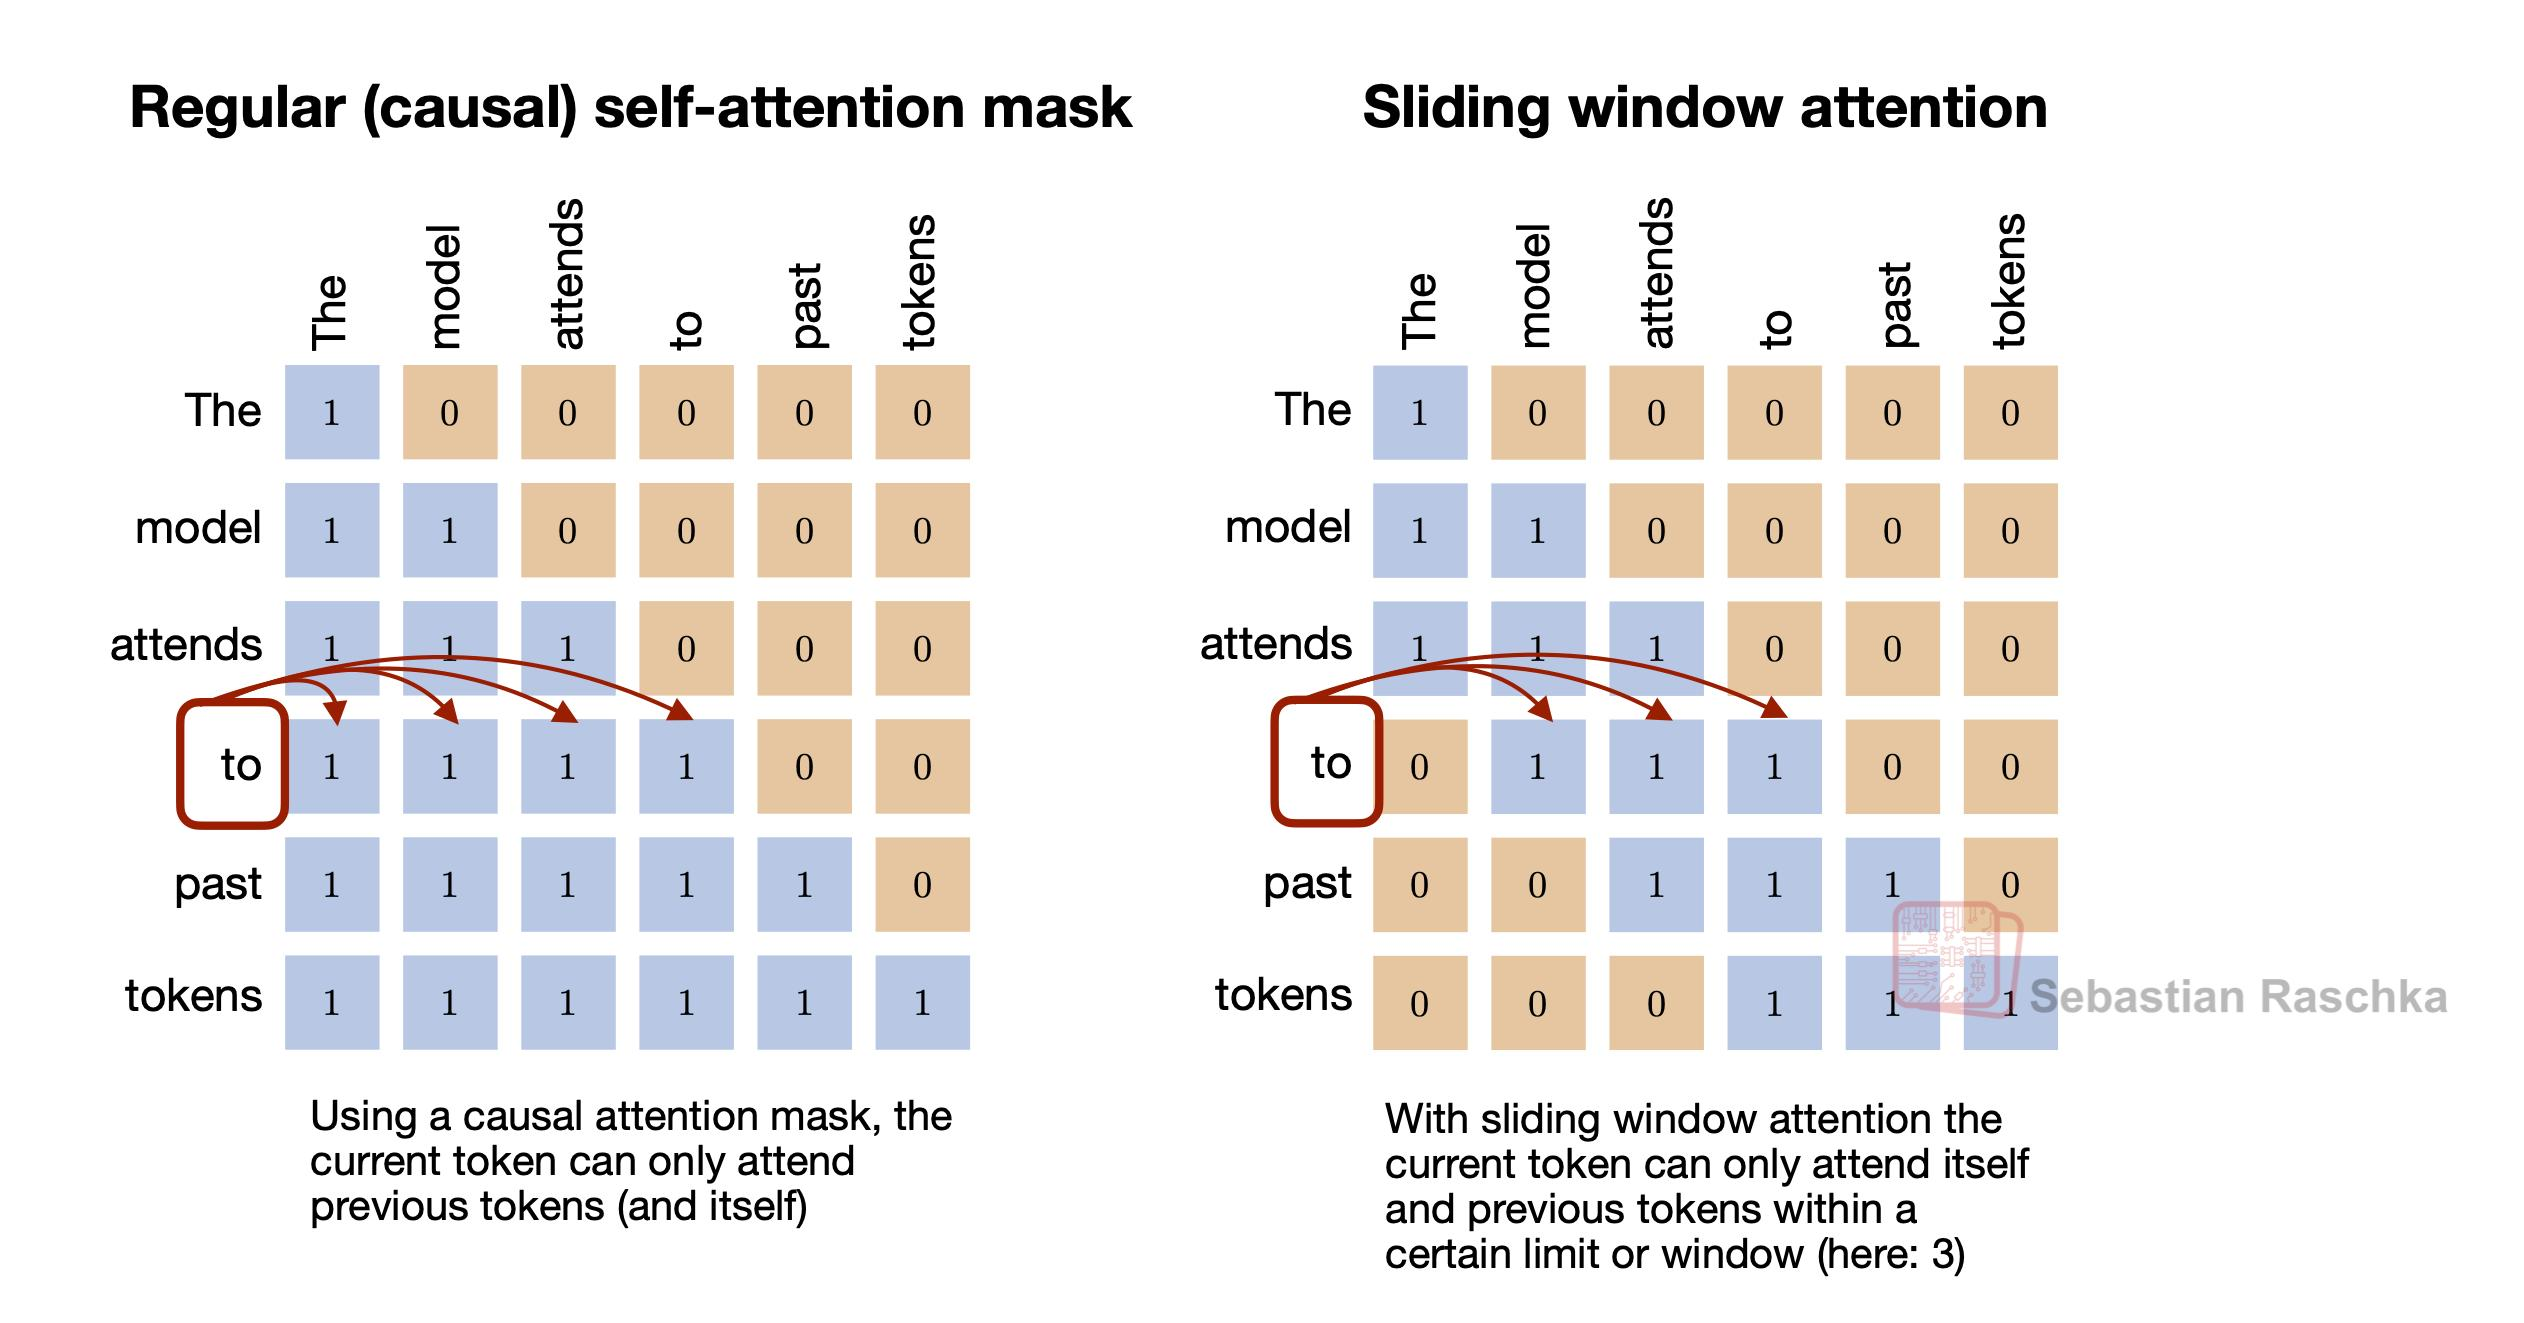
\includegraphics[width=0.8\textwidth]{nsa-sliding.png}
    \caption{NSA 的滑动窗口注意力分支}
    \label{fig:nsa-sliding}
  \end{figure}

  \item \textbf{Gated Aggregation（门控融合）}

  三条分支分别计算 Attention Output，最后通过可学习的 Gate 进行加权融合：
  \[
    O_t = \sum_{c\in\{cmp,slc,win\}} g_t^{c} O_t^{c}
  \]
\end{enumerate}

\subsection{DSA}

DSA（DeepSeek Sparse Attention）可以认为是 NSA 的升级 pro max 版本，其基本思想和 NSA 一致，大致也是分为两个阶段：\textbf{注意力压缩}和\textbf{注意力选择}。在 DSA 中，我们用 MLA 来处理注意力压缩的部分，用 Indexer 来做注意力选择的部分，这两个组件都有相当的复杂度，Indexer 我们在后续章节有统一的深入介绍，在这里我们可以着重介绍下 MLA，窥探下压缩注意力可以被玩出多少花样。

\subsubsection{MLA}

\begin{figure}[htbp]
  \centering
  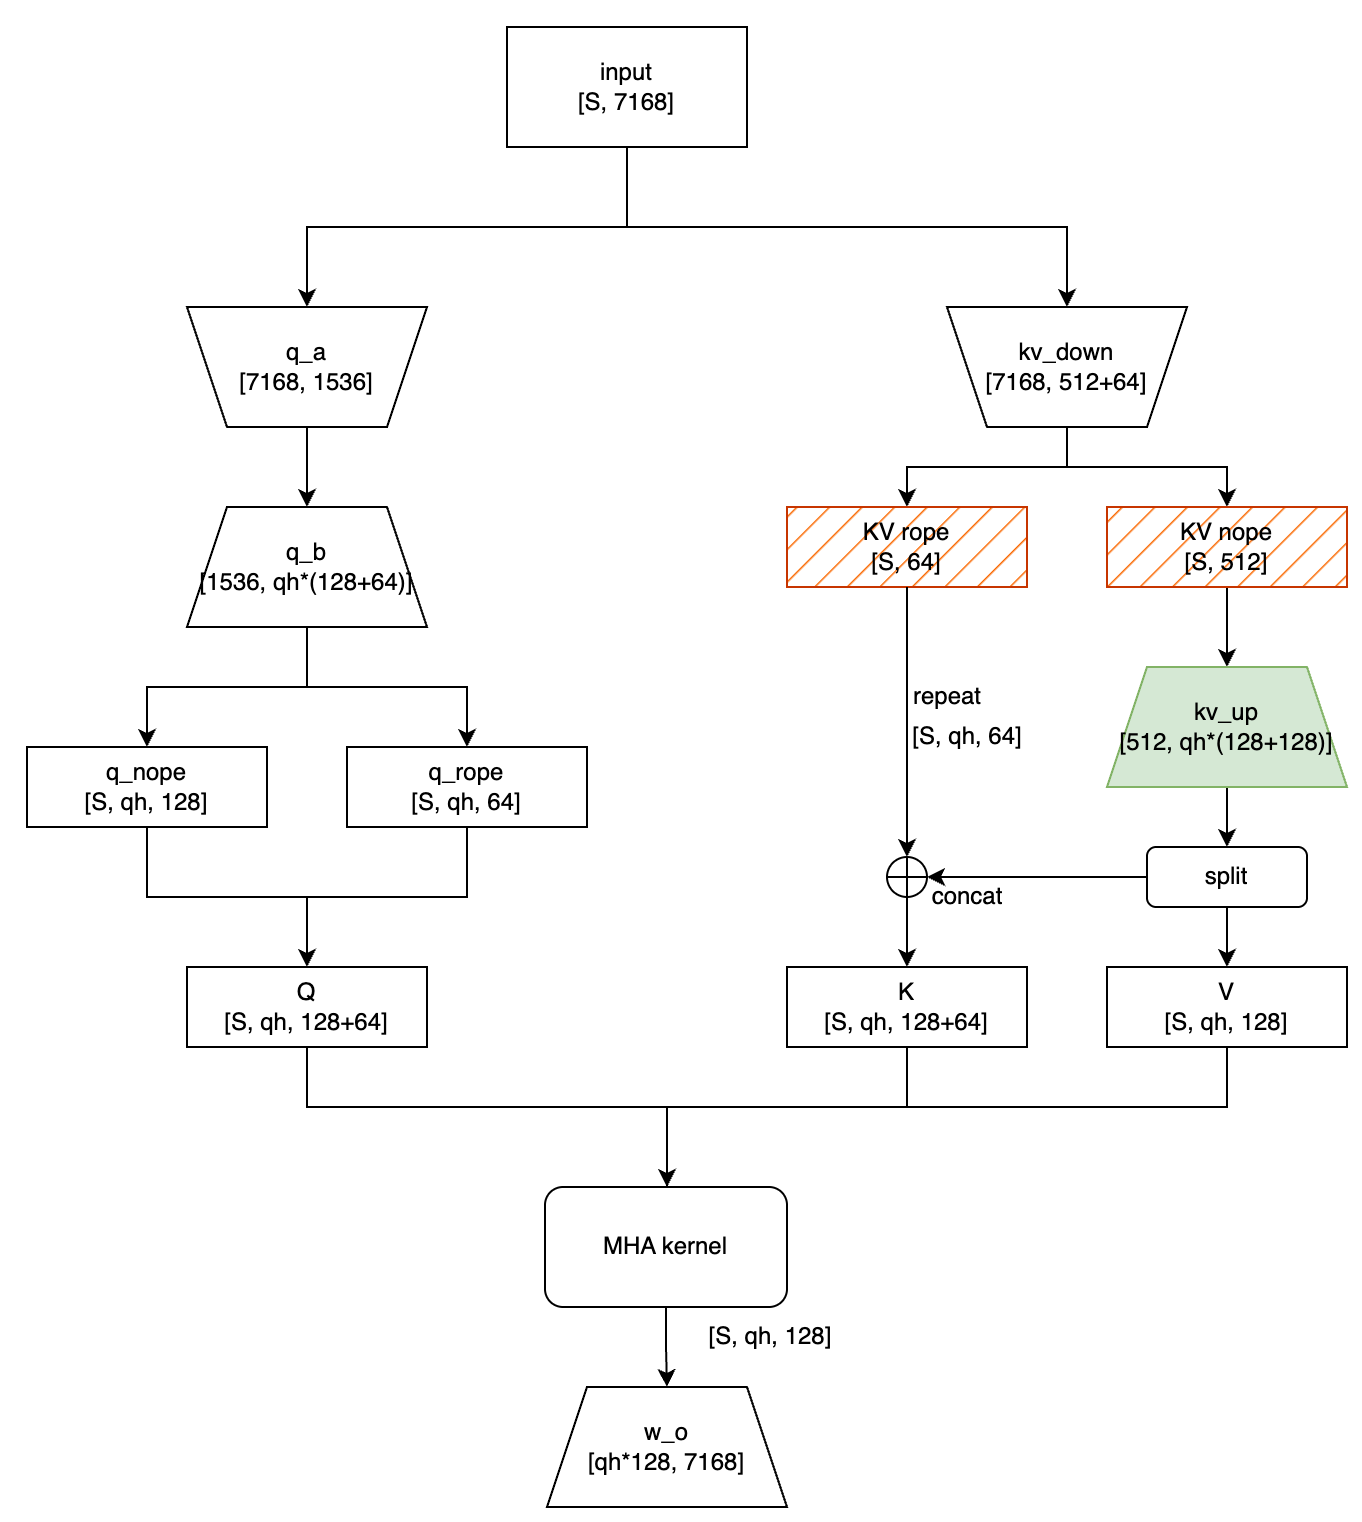
\includegraphics[width=0.85\textwidth]{kv-path.png}
  \caption{MLA 的 KV 通路}
  \label{fig:kv-path}
\end{figure}

\textbf{KV 通路（KV Path）可以拆成三步：}

\begin{enumerate}
  \item \textbf{下采样，生成紧凑的 KV 表示：input $\to$ kv\_down}

  记当前 Token 在这一层 Attention 的输入向量为 $h$。它先经过 kv\_down 下采样，得到一份紧凑表示，供后续构造 K 和 V。

  \item \textbf{将内容与 RoPE 分量分成两路：kv\_down $\to$ kv nope / kv rope $\to$ kv\_up}

  kv\_down 的输出维度是 $512 + 64$，分为 KV nope 和 KV rope 两部分。

  \begin{itemize}
    \item 前 512 维是内容潜向量 $c$（KV nope），用于生成各 Head 的内容 K 和 V，后续可由 kv\_up 展开得到（可以记为 $Ac$，$A$ 是一个上采样矩阵），此时展开具有 head 维度，也就是图上的 qh；
    \item 后 64 维是用于位置打分的 Key 分量（KV rope），经 RoPE 旋转后得到 $k_{pe}$。
  \end{itemize}

  \item \textbf{产出 K/V}

  \begin{itemize}
    \item 展开后的 kv 再按照 dim 维度 split 得到一份 K 和 V，形状均为 $(S, qh, 128)$；
    \item V 就是最终的 V，而对于 K 来说，我们需要对前面的 $k_{pe}$ 按照 head 维度广播得到 $(S, qh, 64)$，再与上面得到的 K 拼接得到最终的 K，形状为 $(S, nh, 192)$。
  \end{itemize}
\end{enumerate}

\textbf{Q 通路（Q Path）与 Attention 计算：}

\begin{enumerate}
  \item \textbf{下采样与上采样，生成 Q：input $\to$ q\_down $\to$ q\_up}

  输入向量 $h$（形状 \texttt{(S, d\_model)}）先经过 \texttt{q\_down} 下采样，再经过 \texttt{q\_up} 上采样并按 Head 拆分，得到形状为 \texttt{(S, qh, 192)} 的张量。

  \item \textbf{拆分内容与 RoPE 分量，组装 Q}

  将每个 Head 的 192 维沿最后一维 split 为两部分：

  \begin{itemize}
    \item 前 128 维为内容分量 $q_{nope}$，形状 \texttt{(S, qh, 128)}，不做 RoPE；
    \item 后 64 维为位置分量 $q_{rope}$，形状 \texttt{(S, qh, 64)}，施加 RoPE 旋转后与 $q_{nope}$ 重新拼接，得到最终的 $Q$，形状为 \texttt{(S, qh, 192)}。
  \end{itemize}

  \item \textbf{Attention 计算与汇总 V}

  将组装好的 $Q$、$K$ 和 $V$ 送入 Attention kernel。$Q$ 与 $K$ 做点积时，内容分量与位置分量各自相乘再相加；V 本身不做 RoPE 旋转，位置信息通过注意力权重影响 V 的汇总，这个过程可以用以下公式表示：
  \[
    Q = [q_{nope}; q_{rope}], \qquad K = [Ac; k_{pe}]
  \]
  \[
    Q^\top K = q_{nope}^\top (Ac) + q_{rope}^\top k_{pe}
  \]
  两项相加并经过缩放（Scale）和 Softmax，得到 \texttt{(qh, S, S)} 的注意力权重矩阵；再用该权重对 $V$ 加权求和，得到输出 \texttt{(S, qh, 128)}，最后经 \texttt{o\_proj} 投影回 \texttt{(S, d\_model)}。
\end{enumerate}

\subsubsection{Indexer}

前面提到，DSA 把主 Attention 的交互量从全量 $O(L^2)$ 降到了每个 Query 只取 $k = 2048$ 个 Token，而负责“挑出这 2048 个位置”的组件就是 \textbf{Lightning Indexer}。

\begin{figure}[htbp]
  \centering
  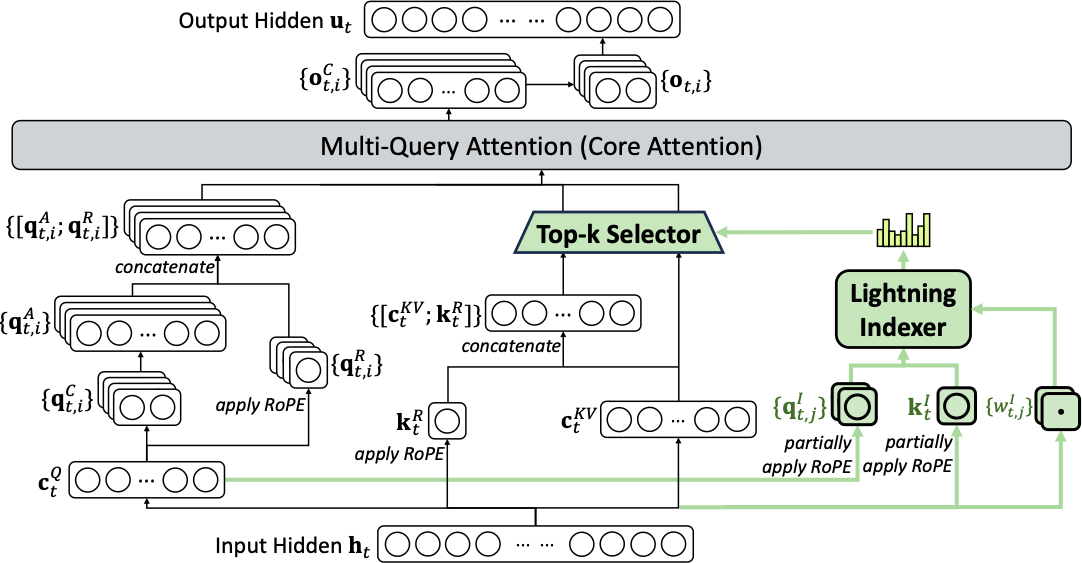
\includegraphics[width=0.85\textwidth]{v32-arch.png}
  \caption{V3.2 的 DSA 架构与 Indexer}
  \label{fig:v32-arch}
\end{figure}

\textbf{打分方式：ReLU + MQA 轻量索引 + FP8}

对于当前 Query Token $h_t$ 和历史 Token $h_s$，Indexer 计算相关性分数的公式如下：
\[
  I_{t,s} = \sum_{j=1}^{H^I} w_{t,j}^I \cdot \text{ReLU}\left(q_{t,j}^I \cdot k_s^I\right)
\]
这里的索引向量 $q_{t,j}^I \in \mathbb{R}^{d^I}$、$k_s^I \in \mathbb{R}^{d^I}$ 以及头权重 $w_{t,j}^I$ 具体是这样算出来的：

\begin{itemize}
  \item \textbf{Q 侧 $q_{t,j}^I$（复用 MLA \texttt{q\_down}）}：Indexer 不从原始输入 $h_t$ 重新做一次下采样，而是直接复用主 MLA 通路里 \texttt{q\_down} 产出的压缩表示 $c_t^Q$，经过线性投影 \texttt{wq\_b} 展开为多头，形状为 \texttt{(S, H\textasciicircum I, d\textasciicircum I)}。随后沿最后一维拆成位置部分和内容部分，只对位置部分（如前 64 维）施加 RoPE 旋转再拼回。
  \item \textbf{K 侧 $k_s^I$（单头共享，MQA 风格）}：从输入 $h_s$ 经 \texttt{wk} 线性投影到 \texttt{(S, d\textasciicircum I)} 并做一次 LayerNorm（注意只有 1 个 Head，所有 $H^I$ 个 Indexer Query Head 共享这同一份 $k_s^I$，大幅压低缓存和访存开销）。同样拆出位置分量施加 RoPE 后拼回。
  \item \textbf{Hadamard 旋转 + FP8 量化}：为了压低全历史扫描的计算与显存成本，计算出来的 $q$ 和 $k$ 会先经过一次 Hadamard 旋转（平滑特征分布、减少离群值），再按块量化为 FP8（\texttt{e4m3}）；历史 Token 的 \texttt{k\_fp8} 和量化 scale 会直接存入独立的 Indexer Cache。
  \item \textbf{头权重 $w_{t,j}^I$ 与 ReLU 打分}：输入 $h_t$ 经线性层 \texttt{weights\_proj} 算出每个 Head 的标量权重（并乘上维度与量化缩放因子），最后通过融合 Kernel 在 FP8 下计算 $\sum_j w_{t,j}^I \cdot \text{ReLU}(q_{t,j}^I \cdot k_s^I)$。用 ReLU 替代 Softmax 可以避免沿历史序列做全局归约同步，吞吐更高。
\end{itemize}

\textbf{细粒度 Token 选择：}

拿到所有历史位置的分数 $\{I_{t,s}\}$ 后，直接按 Top-$k$ 选出得分最高的 2048 个历史位置，只把这些位置对应的潜向量 $c_s$ 和位置 Key $k_{pe,s}$ 送入主 MLA 做精确计算。

\textbf{两阶段训练：}

Indexer 刚接上时还不知道该选哪些位置，所以 DeepSeek-V3.2 在 V3.1-Terminus 的基础上分两步继续预训练：先在 Dense Attention 下单独训 Indexer，再切到稀疏模式一起训。

\begin{table}[htbp]
  \centering
  \small
  \begin{tabular}{p{2.8cm}p{5.6cm}p{6.6cm}}
    \hline
    \textbf{} & \textbf{Dense Warm-up} & \textbf{Sparse Training} \\
    \hline
    主 Attention & Dense & Top-$k$ 稀疏，$k = 2048$ \\
    \hline
    训练的参数 & 只有 Indexer，主模型冻结 & 主模型和 Indexer \\
    \hline
    Indexer 的 loss & 在全部历史位置上算 KL & 只在选中的位置 $\mathcal{S}_t$ 上算 KL \\
    \hline
    主模型的 loss & 无 & 语言模型 loss \\
    \hline
    学习率 & $10^{-3}$ & $7.3 \times 10^{-6}$ \\
    \hline
    训练量 & 1000 步 $\times$ 16 条 128K 序列，约 2.1B tokens & 15000 步 $\times$ 480 条 128K 序列，约 943.7B tokens \\
    \hline
  \end{tabular}
\end{table}

KL 的目标分布 $p_{t,:}$ 来自主 Attention：把所有 Head 的注意力分数加起来，再沿序列维做 L1 归一化。第二阶段里 Indexer 的输入从计算图上 detach 掉，Indexer 只接收 KL 的梯度，主模型只接收语言模型 loss 的梯度，两边互不影响。

\subsection{Sliding shift 神鬼二象性}

不管是 NSA 里的 Compression 分支，还是各类分块 KV-Cache 压缩方案（例如 DeepSeek-V4 中的 CSA），只要按固定步长（stride $S$）把连续的一段 Token 压成少数几个缓存条目，就会引入一个原本不存在的新位置坐标——\textbf{相位（Phase）}，即 Token 落在压缩周期内的相对偏移量（$t \bmod S$）。

\begin{figure}[htbp]
  \centering
  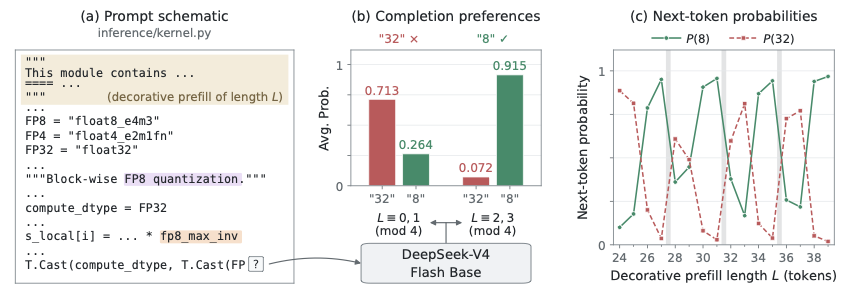
\includegraphics[width=0.85\textwidth]{phase-headline.png}
  \caption{分块压缩引入的相位坐标}
  \label{fig:phase-headline}
\end{figure}

最近的工作揭示了这种稀疏压缩架构下的一个系统性缺陷：\textbf{相位敏感性（Phase Sensitivity）}。同一段代码或关键信息，仅仅因为前面多加或少减了几个无关字符（即发生 Sliding Shift，改变了目标信息相对于压缩窗口边界的相位），模型在长上下文检索任务上的准确率就会出现高达 \textbf{40 个百分点}的周期性波动（在可控预训练实验中甚至可达 78 个百分点），且波动周期严格等于压缩步长 $S$（如 DeepSeek-V4 的 $S=4$、V4.1 的 $S=2$）。

\begin{figure}[htbp]
  \centering
  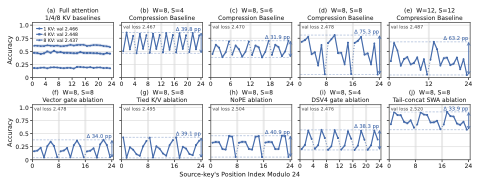
\includegraphics[width=0.85\textwidth]{phase-accuracy.png}
  \caption{检索准确率随相位的周期性波动}
  \label{fig:phase-accuracy}
\end{figure}

结合稀疏注意力的结构特性与论文的因果干预实验，这种“神鬼二象性”背后的机制可以拆解为两点：

\begin{enumerate}
  \item \textbf{压缩门控的“静态相位特化”（Phase Specialization）}

  在分块压缩稀疏注意力中，每个压缩窗口需要通过门控权重 $\alpha_{j,i}$ 把窗口内不同偏移位置 $i$ 的 Token 聚合成一条缓存条目。论文通过 KV-Head Knockout（均值替换）和门控熵分析发现：在预训练过程中，许多注意力头的压缩门控会自发收敛成\textbf{静态偏移偏好}（Static Concentration）——即不管输入内容是什么，某些头固定只给窗口早期偏移（如 $i=0,1$）赋高权重，另一些头固定只关注窗口中段或尾部。这意味着单个 Head 实际上只负责“打捞”特定相位的历史信息；当目标信息因为 Sliding Shift 落到该 Head 的低权重相位上时，就必须依赖其他 Head 接力，一旦某几个相位缺乏足够多的特化 Head 覆盖，就会形成周期性的检索盲区。

  \begin{figure}[htbp]
    \centering
    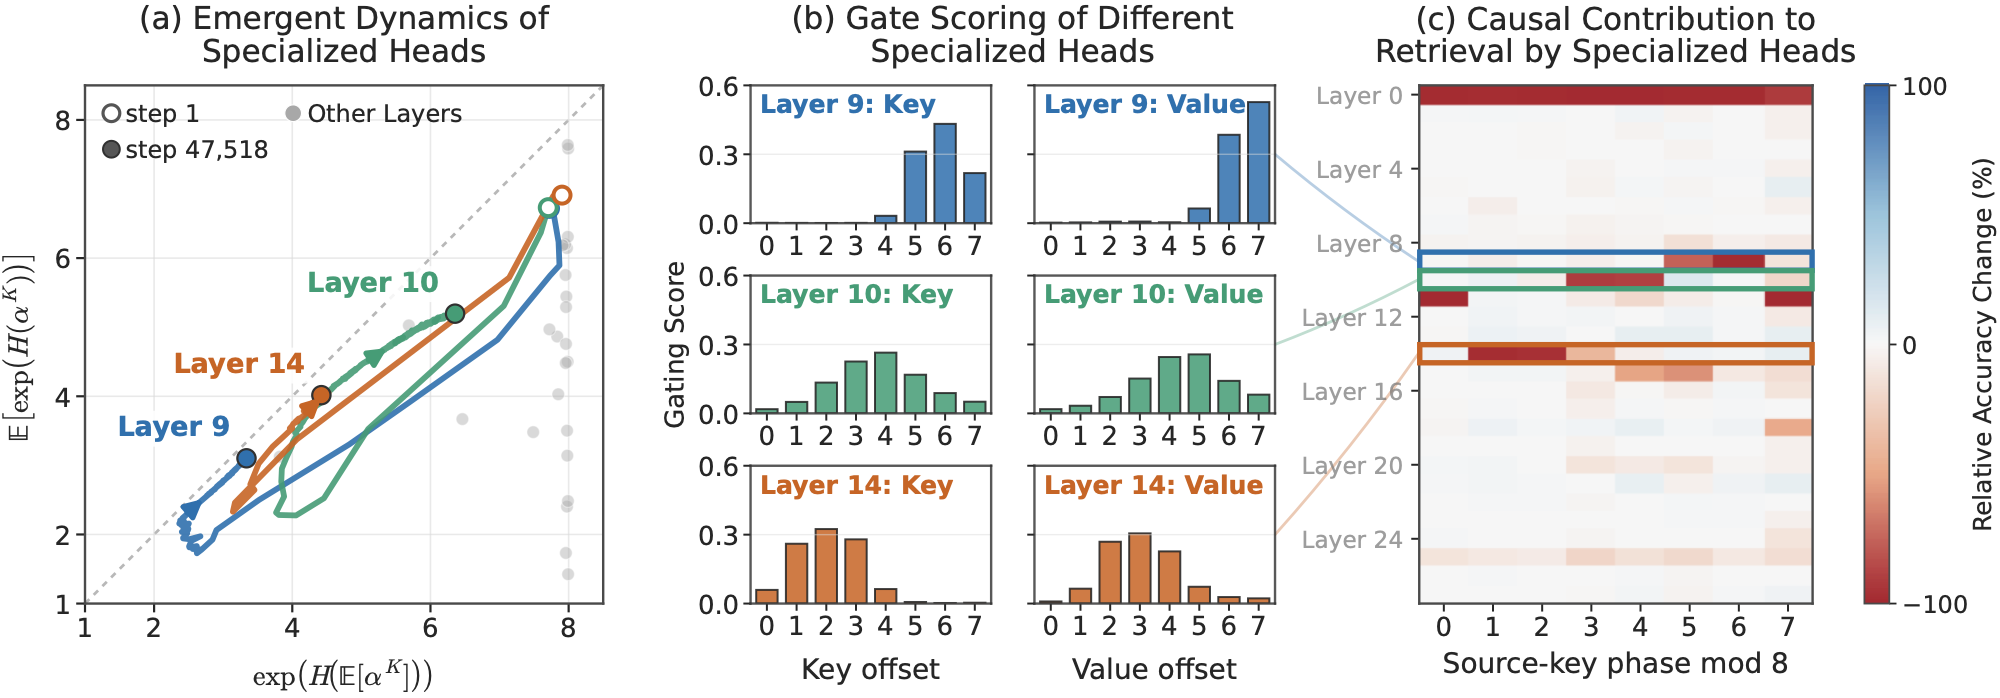
\includegraphics[width=0.8\textwidth]{specialization.png}
    \caption{Key 门控收敛到窗口的早、中、晚三个偏移段}
    \label{fig:specialization}
  \end{figure}

  \item \textbf{周期由步长 $S$ 决定，而非仅由窗口边界决定}

  很多人直觉上认为精度波动是因为“Key 和 Value 刚好被窗口边界劈开”，但论文的对照实验推翻了这一单一归因：即使在 $W=8, S=8$ 且 Key-Value 同处一个窗口内部的相位（0--6）之间，检索准确率依然有超过 50 个百分点的落差；而且当窗口重叠（$W=8, S=4$）时，波动周期依然跟随步长 $S=4$ 而非窗口大小 $W=8$。

  \begin{figure}[htbp]
    \centering
    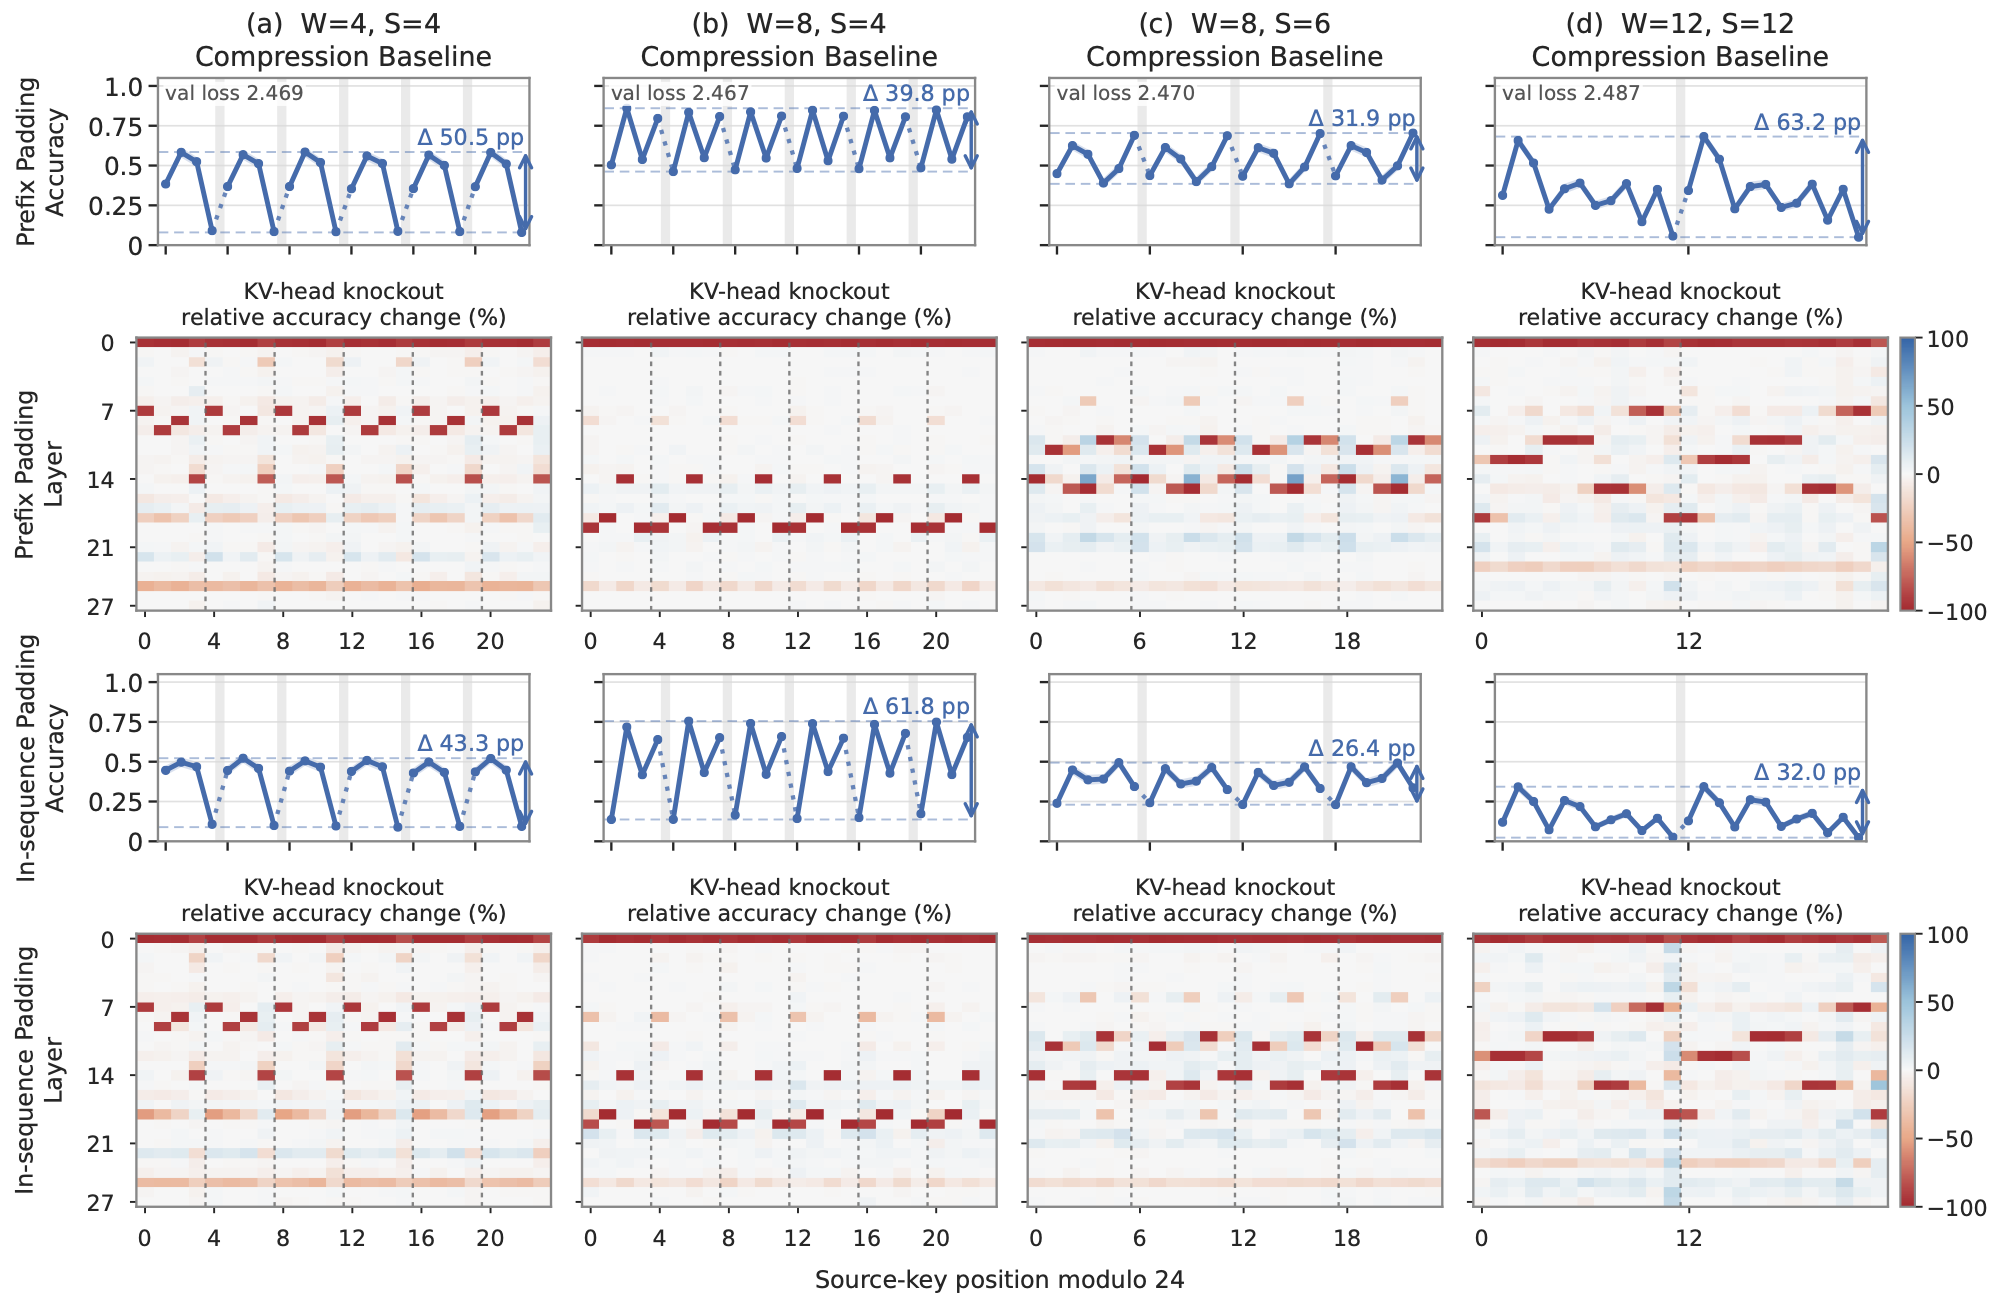
\includegraphics[width=0.8\textwidth]{group-geometry.png}
    \caption{不同 $W$、$S$ 组合下的周期对照}
    \label{fig:group-geometry}
  \end{figure}

  这说明问题出在稀疏压缩“按固定步长离散采样并有损聚合”的读写机制本身：只要存在固定步长 $S$ 的块级压缩，常规 Benchmark 的平均分就会掩盖掉这些周期性弱点（Weak Spots），而类似 NSA 的滑动窗口分支也只能兜底最近邻，无法消除远距离压缩记忆的相位盲区。
\end{enumerate}

\subsection{开销分析}

我们可以把标准 Dense Attention、NSA 和 DSA 放在同一口径下做一次横向对比（记序列长度为 $L$，单个 Token 维度为 $d$）：

\begin{table}[htbp]
  \centering
  \small
  \begin{tabular}{p{2.5cm}p{3.5cm}p{4.4cm}p{4.4cm}}
    \hline
    \textbf{维度} & \textbf{标准 Dense Attention (GQA)} & \textbf{NSA} & \textbf{DSA (基于 MLA)} \\
    \hline
    主 Attention 计算复杂度 & $O(L^2)$ & 压缩 $O(L^2/s)$ + 选择 $O(L \cdot n B)$ + 滑窗 $O(Lw)$ & $O(Lk)$（$k=2048$ 固定） \\
    \hline
    总计算复杂度 & $O(L^2)$ & 亚二次，但压缩分支仍随 $L$ 增长 & 含 $O(L^2)$ 项（FP8 Indexer 扫全历史，但系数极小） \\
    \hline
    KV Cache 显存占用 & 随 $L$ 线性增长 & 随 $L$ 线性增长（需存完整原始 KV + 压缩块 KV） & 随 $L$ 线性增长（仅存 \texttt{512+64} 潜向量 + 极小 Indexer Key） \\
    \hline
    单步 Decode 访存量 & 读取全部历史 KV & 读取全部压缩块 + Top-$n$ 块 + 滑窗 & 读取全部 Indexer Key + 筛选出的 $k$ 个潜向量 \\
    \hline
    精度损失来源 & 无（基线） & 块级打分粗粒度误差、块边界相位敏感性 & 无独立全局信息，完全依赖 Indexer 的 Top-$k$ 召回率 \\
    \hline
  \end{tabular}
\end{table}

可以看到，稀疏注意力省下的主要是\textbf{主 Attention 的计算量与单步访存带宽}，而\textbf{静态显存依然随上下文长度 $L$ 线性增长}。其中 DSA 通过与 MLA 结合，把单个 Token 的缓存压到 576 维，同时把昂贵的全量交互转移到 FP8 轻量 Indexer 上，在长序列 Prefill 与 Decode 阶段都拿到了明显的成本下降：

\begin{figure}[htbp]
  \centering
  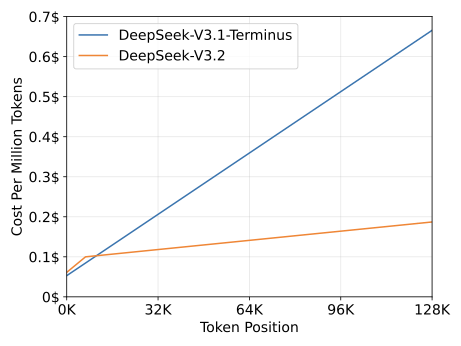
\includegraphics[width=0.75\textwidth]{cost-prefilling.png}
  \caption{Prefill 推理成本对比}
  \label{fig:cost-prefilling}
\end{figure}

\begin{figure}[htbp]
  \centering
  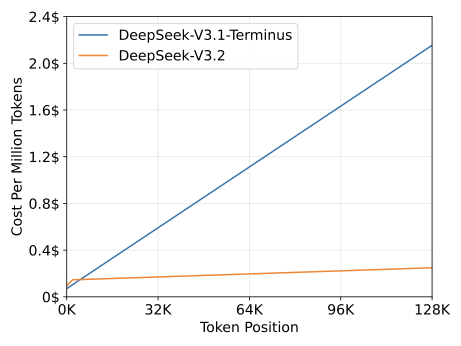
\includegraphics[width=0.75\textwidth]{cost-decoding.png}
  \caption{Decode 推理成本对比}
  \label{fig:cost-decoding}
\end{figure}

\subsection{Infra 层面的挑战}

稀疏注意力在算法纸面上把复杂度降了下来，但落到推理引擎和 GPU 硬件上，工程比 Dense Attention 复杂不少：

\begin{table}[htbp]
  \centering
  \small
  \begin{tabular}{p{2.8cm}p{5.8cm}p{6.4cm}}
    \hline
    \textbf{挑战点} & \textbf{核心矛盾} & \textbf{工程应对思路} \\
    \hline
    非连续访存与 Tensor Core & FlashAttention 依赖规则 Tile 连续搬运；稀疏筛选导致地址离散、Batch 内分化 & Decode 阶段采用 MQA 模式（同 Token 多 Head 共享选中 KV 提升访存复用） \\
    \hline
    Paged / Prefix Cache 适配 & 逻辑 Token 索引必须经过页表映射；前缀共享需兼顾压缩块边界与 Indexer Key 缓存 & 维护逻辑索引到物理页的映射表，对齐固定块粒度以支持前缀复用 \\
    \hline
    KV Offload 与分布式通信 & 必须先算完 Indexer 才知道要搬哪些 KV 页，无法做确定性流水线预取 & 优化异步 DMA 与跨节点通信重叠，将热点页常驻 HBM \\
    \hline
    短序列下的负优化 & 短序列时 Indexer + Top-$k$ + 离散调度的开销高于直接算全量 Attention & 设置长度阈值，短序列 Prefill 直接回退到 Masked MHA 路径 \\
    \hline
  \end{tabular}
\end{table}

\section{线形注意力}

与稀疏注意力“保留全量 KV Cache、每次挑一部分来算”的思路不同，线形注意力（Linear Attention）选择了另一条路：\textbf{不再保存随长度线性膨胀的历史 KV，而是把所有历史信息持续压缩进一个固定大小的状态矩阵中。}
\[
  S_t \in \mathbb{R}^{d_k \times d_v}
\]
这样一来，Decode 阶段每生成一个新 Token 只需要读取并更新这一个固定状态，单步计算量和显存占用都是严格 $O(1)$，整段序列的复杂度是真正的 $O(L)$。

早期的线形注意力（例如直接用核函数去掉 Softmax，写成 $S_t = S_{t-1} + k_t v_t^\top$）虽然复杂度降下来了，但精度一直打不过标准 Attention。核心原因在于\textbf{状态容量有限}：只做纯加法累加，历史信息会不断堆积在有限的矩阵空间里，新旧记忆互相覆盖干扰（Memory Interference），既忘不掉过期的噪音，也很难精准更新或覆盖某条旧信息。

\subsection{GDN}

\textbf{GDN（Gated DeltaNet）}是这一轮线形注意力复兴中的代表性架构，它把两条原本独立的技术思路结合在了一起：\textbf{Mamba2 的数据依赖门控衰减（Gating）}和 \textbf{DeltaNet 的纠错式写入规则（Delta Rule）}。

\textbf{状态更新与在线学习视角：}

它的状态更新公式可以写为：
\[
  S_t = \alpha_t \left(I - \beta_t k_t k_t^\top\right) S_{t-1} + \beta_t v_t k_t^\top
\]
把后面两项合并改写一下，物理意义会更直观：
\[
  S_t = \alpha_t S_{t-1} + \beta_t \left(v_t - \alpha_t S_{t-1} k_t\right) k_t^\top
\]
从在线回归（Test-Time SGD）的角度来看，状态矩阵 $S$ 就像一个在推理时不断用梯度下降更新的快权重（Fast Weight）：

\begin{itemize}
  \item \textbf{全局门控衰减 $\alpha_t \in (0, 1)$}：等价于自适应的权重衰减（Weight Decay）。当上下文切换或旧记忆不再重要时，模型把 $\alpha_t$ 调小，整体缩放历史状态 $S_{t-1}$ 以腾出容量。
  \item \textbf{Delta Rule 精确纠错写入}：在写入新键值对 $(k_t, v_t)$ 之前，先用当前的 $k_t$ 去旧状态里查询已经存了什么（$\alpha_t S_{t-1} k_t$），算出目标值 $v_t$ 与旧记忆之间的残差（Delta），再按学习率 $\beta_t \in (0, 1)$ 把差值更新进去。这相当于“先擦除旧值、再写入新值”，大幅降低了不同 Key 之间的记忆碰撞。
\end{itemize}

这两者的互补性在长文本检索对比中体现得很明显：纯 DeltaNet 缺乏遗忘机制，在真实文本噪声下容易发生记忆碰撞；纯 Mamba2 只有指数衰减而没有精确擦除，长程保留能力迅速退化；GDN 把两者结合后，在 1K--8K 序列检索上同时守住了记忆保留与干扰过滤。

\textbf{Chunkwise Parallel（分块并行）：}

如果直接按上面公式做串行递推，无法利用 GPU Tensor Core。GDN 依托分块并行算法，将长度为 $L$ 的序列切分为若干大小为 $C$ 的 Chunk：

\begin{itemize}
  \item \textbf{Chunk 内部}：把连续 $C$ 步的 Rank-1 更新打包成矩阵形式（基于 WY 表示），利用矩阵乘法在 Tensor Core 上并行计算输出；
  \item \textbf{Chunk 之间}：只传递每个 Chunk 末尾的状态矩阵 $S_{[t]}$，在保留 $O(1)$ 推理显存的同时，维持高训练与 Prefill 吞吐。
\end{itemize}

\subsection{KDA}

\textbf{KDA（Kimi Delta Attention）}是 Kimi 在 Kimi Linear / Kimi K3 中提出的改进版线形注意力。

\begin{figure}[htbp]
  \centering
  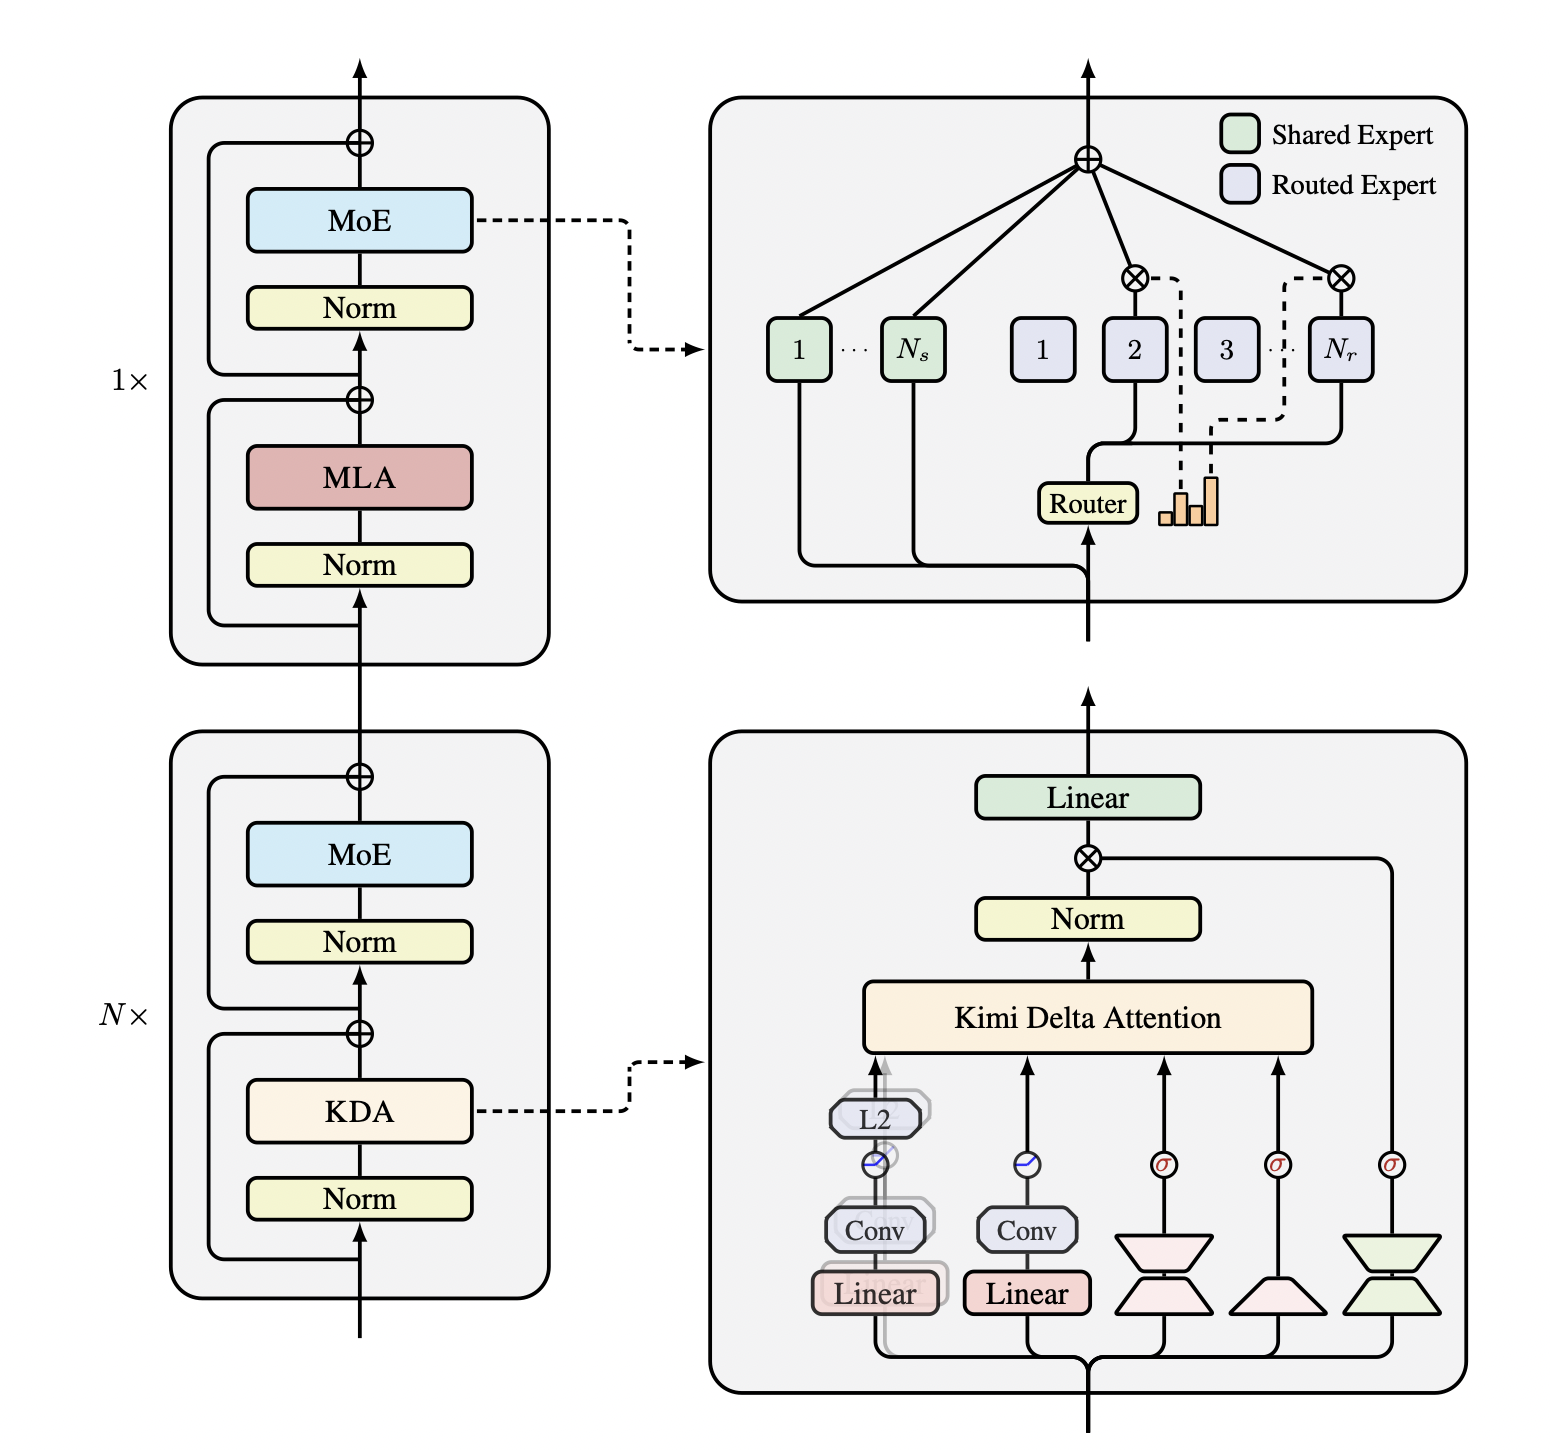
\includegraphics[width=0.85\textwidth]{kda-arch.png}
  \caption{KDA 架构}
  \label{fig:kda-arch}
\end{figure}

\textbf{从标量衰减到逐通道对角衰减：}

在 GDN 中，每个 Head 只有一个标量 $\alpha_t$，同一个 Head 内的所有特征维度必须以完全相同的速度一起遗忘。KDA 将标量 $\alpha_t$ 替换为\textbf{逐通道（Channel-wise）的对角衰减矩阵} $\operatorname{Diag}(\alpha_t)$：
\[
  S_t = \left(I - \beta_t k_t k_t^\top\right)\operatorname{Diag}(\alpha_t) S_{t-1} + \beta_t k_t v_t^\top
\]
这样一来，同一个 Head 内部的不同特征通道可以各自拥有独立的遗忘速率：部分通道保持接近 1 的衰减率用来长期记忆全局设定或主题，另一部分通道则可以用较小的衰减率快速刷新局部语法或临时变量。

\textbf{工程参数化与硬件效率（DPLR 特化）：}

\begin{itemize}
  \item \textbf{输入与门控设计}：$q, k, v$ 在线性投影后均经过 ShortConv 与 Swish 激活，其中 $q, k$ 额外做 L2Norm 以保证状态转移矩阵特征值的数值稳定性；通道衰减 $\alpha_t$ 与输出门控均采用低秩投影（Low-rank Projection）参数化，输出前配合 Head-wise RMSNorm 与 Sigmoid 门控以缓解 Attention Sink。
  \item \textbf{WY + UT 变换优化}：引入对角衰减后，状态转移矩阵属于 DPLR（Diagonal-Plus-Low-Rank）形式，传统做法（如 GLA）为了数值稳定需要在对数域做全精度二次分块，无法吃满半精度 Tensor Core。KDA 通过将 $a, b$ 向量同时绑定到 $k$ 上，并结合 WY 表示与 UT 变换消除了多余的矩阵求逆与二次分块乘法，使算子效率相比通用 DPLR 提升约 \textbf{100\%}。
\end{itemize}

\begin{table}[htbp]
  \centering
  \small
  \begin{tabular}{p{2.3cm}p{2.5cm}p{3.5cm}p{2.9cm}p{3.3cm}}
    \hline
    \textbf{架构} & \textbf{衰减门控形式} & \textbf{写入更新规则} & \textbf{遗忘粒度} & \textbf{硬件实现关键} \\
    \hline
    早期线性注意力 & 无衰减 & 纯加法累加 & 无遗忘（易饱和） & 标准矩阵乘 / 累加 \\
    \hline
    GDN & 标量 $\alpha_t$ & Delta Rule 纠错写入 & Head 级统一遗忘 & Chunkwise Parallel \\
    \hline
    KDA & 向量 $\operatorname{Diag}(\alpha_t)$ & Delta Rule 纠错写入 & Channel 级独立遗忘 & Chunkwise WY + UT 变换融合 Kernel \\
    \hline
  \end{tabular}
\end{table}

\textbf{与 MLA 的混合（3:1 + NoPE）：}

在 Kimi Linear 架构中，KDA 采用 \textbf{3 层 KDA + 1 层 Full MLA} 的层间交替混合（3:1 比例），并且对 MLA 层采用 \textbf{NoPE（无位置编码）}——将位置编码与近邻偏置完全交给 KDA 层承担。这样既免去了长上下文场景下对 RoPE 的频率外推调参（如 YaRN），也让 MLA 层在推理时可以直接转为纯 MQA 模式，在 1M 上下文下减少最多 \textbf{75\%} 的 KV Cache 占用，并带来最高 \textbf{6 倍}的解码吞吐提升。

\subsection{开销分析}

与稀疏注意力不同，线形注意力真正把\textbf{计算复杂度}和\textbf{状态显存}都压到了线性 / 常数级别。以 Kimi Linear 论文给出的理论 FLOPs 口径为例（设序列长度为 $T$，单头维度为 $d_h$，分块大小 $C=64$）：
\[
  \text{FLOPs}_{\text{KDA}}(T; C, d_h) = 6 T d_h^2 + 3 T C d_h + T C^2, \qquad \text{FLOPs}_{\text{Attn}}(T; d_h) = 2 T^2 d_h
\]
在 $d_h = 128, C = 64$ 时，当序列长度超过约 500 个 Token，KDA 的计算量就会低于标准全注意力；到 128K--1M 级长上下文时，差距会拉开几个数量级。

\begin{table}[htbp]
  \centering
  \small
  \begin{tabular}{p{2.5cm}p{3.3cm}p{4.6cm}p{4.4cm}}
    \hline
    \textbf{维度} & \textbf{Full Attention (MLA)} & \textbf{纯 GDN / KDA} & \textbf{混合架构 (Kimi Linear 3:1)} \\
    \hline
    Prefill 计算量 & $O(T^2 d_h)$ & $O(T d_h^2 + T C d_h)$ & 75\% 线性层 + 25\% MLA（1M 下整体提速 $2.9\times$） \\
    \hline
    单步 Decode 访存 & 读取全量历史 KV（随 $T$ 线性增长） & 读取固定状态矩阵 $S_t \in \mathbb{R}^{128 \times 128}$（$O(1)$） & 仅 25\% 的层需读历史 KV，I/O 瓶颈向 3:1 逼近 \\
    \hline
    单 Token / 状态显存 & 随 $T$ 线性膨胀 & 恒定 $O(1)$（不随序列长度增长） & KV Cache 减少最多 75\% \\
    \hline
    Batch 并发扩展性 & 长序列下显存迅速见底，Batch 受限 & 显存释放后可大幅拉大 Batch Size & 1M 上下文下理论解码吞吐提升最高 $6.3\times$ \\
    \hline
  \end{tabular}
\end{table}

\begin{figure}[htbp]
  \centering
  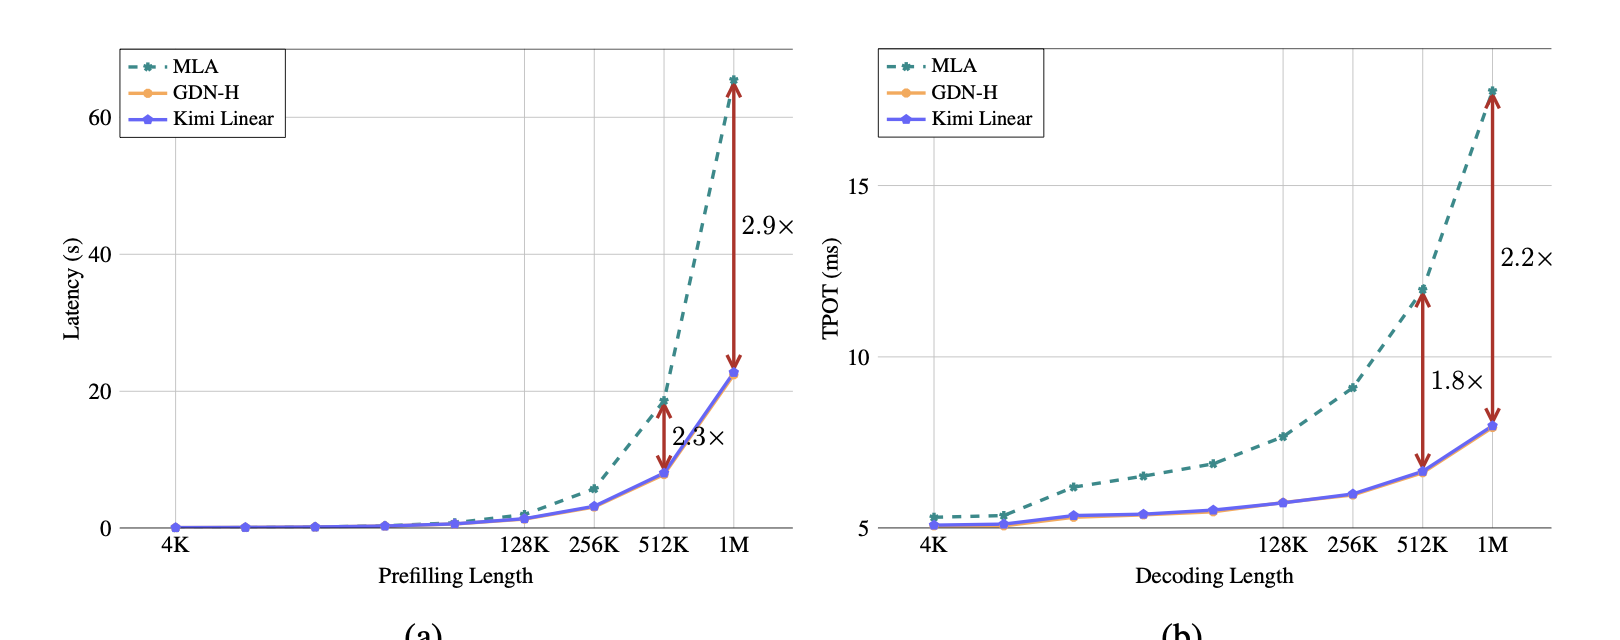
\includegraphics[width=0.75\textwidth]{kda-speed.png}
  \caption{Kimi Linear 与全注意力的解码速度对比}
  \label{fig:kda-speed}
\end{figure}

从实测曲线可以看到（\texttt{batch\_size = 1}）：在 4K--16K 区间，Kimi Linear 与全注意力差距不大；从 128K 开始优势迅速放大，在 1M 长度下 Prefill 延迟降低 $2.9\times$，单请求每 Token 生成时间（TPOT）降低 $2.2\times$。如果把节省下来的显存用来扩大并发 Batch Size，整体解码吞吐可达到全注意力的 $6\times$ 以上。

\subsection{Infra 层面的挑战}

尽管线形注意力在显存和理论 FLOPs 上优势明显，但它打破了传统 Transformer“统一 KV Cache + FlashAttention”的推理基础设施假设，落到生产引擎（如 vLLM / SGLang）上会带来一套全新的工程挑战：

\begin{table}[htbp]
  \centering
  \small
  \begin{tabular}{p{2.8cm}p{5.8cm}p{6.4cm}}
    \hline
    \textbf{挑战点} & \textbf{核心矛盾} & \textbf{工程应对思路} \\
    \hline
    双 Kernel 维护与数值稳定性 & Prefill 需要高算力密度的 Chunkwise 矩阵乘，Decode 需要低延迟的逐 Token 递推；引入对角衰减后 $1/\Gamma$ 易在半精度下溢出 & 分别实现 Triton/CUDA 融合 Chunk Kernel 与 Recurrent Kernel；用绑定 $k$ 的 UT 变换替代通用 DPLR 二次分块 \\
    \hline
    Prefix Cache 与 State 复用 & PagedAttention 按 Token 块复用历史 KV；线性注意力只有压缩后的状态矩阵 $S_t$，无法直接从任意历史 Token 截断恢复 & 在 Chunk 边界（或固定步长）周期性保存状态快照 $S_{[t]}$，设计异构的 State Pool + Paged KV 统一内存管理器 \\
    \hline
    Varlen Batch 与混合层负载不均 & 混合架构中 75\% 线性层显存恒定、算力特征偏矩阵状态更新，25\% MLA 层显存随长度线性增长，两类层在流水线/张量并行下负载不同 & 支持 Ragged Tensor（变长打包）的分块掩码与状态索引隔离，针对线性层与 MLA 层分别规划批处理调度与显存配额 \\
    \hline
    Context Parallel 状态通信 & 标准 Attention 做长序列跨卡切分只需 Ring 传递 KV 块；线性注意力存在严格的时间步因果依赖，后一张卡必须等前一张卡算完末尾状态 & 采用 Chunk 级分布式前缀扫描（Prefix-scan），将跨卡状态矩阵传输与本地 Chunk 内计算流水线重叠 \\
    \hline
  \end{tabular}
\end{table}

\section{走向“共和”与小结}

现在主流的做法（像 Kimi Linear / Kimi K3、Qwen3-Next、MiniMax-01 这些模型）大多是在层与层之间按比例混搭，比如 3 层线形注意力配 1 层全局或稀疏注意力：

\begin{table}[htbp]
  \centering
  \small
  \begin{tabular}{p{3.0cm}p{6.4cm}p{5.6cm}}
    \hline
    \textbf{} & \textbf{线形层（GDN / KDA）} & \textbf{全局 / 稀疏层（MLA / DSA）} \\
    \hline
    占模型层数 & 大头（通常 75\% 左右） & 少数间隔层（如每 4 层插 1 层） \\
    \hline
    缓存形态 & 固定大小状态矩阵 $S_t$ & 历史 KV（或潜在向量 $c$ 与 $k_{pe}$） \\
    \hline
    主要作用 & 处理常规上下文依赖、控制整体显存和吞吐 & 补齐长距离精确召回和细节对齐 \\
    \hline
  \end{tabular}
\end{table}

单独看某一条路线都有硬伤，但 3:1 混在一起之后，KV Cache 直接砍掉四分之三，长距离检索又有少量全局/稀疏层兜住。具体比例和层间怎么搭配还在演进，但“大部分层靠线形降成本、少数层靠全/稀疏保精度”大概率会是接下来长上下文模型的主流形态。


\end{document}
